\chapter{Как появляются периферийные гегемоны}
Почему в античку у римлян была империя, да и вообще у всех вокруг были империи, а у самих греков империй не было? Пожалуй, разжую просто. Прям на пальцах.


Если вы вдруг оказались на окраине цивилизации, в сторонке от Центра Мира, где его древние обитатели меряются писюнами, то не унывайте. Они, канешн, мудрее и культурнее вас, сраных варваров, но у вас есть несколько ключевых преимуществ, которые могут сделать из вас такую крокозябру, как "Периферийного Гегемона". Который ВНЕЗАПНО, за пару поколений, выпрыгнет из ниоткуда и пооткручивает головы всем, в том числе и тем самым светочам цивилизации. Ну а если ваша карта не сыграет, то тоже не переживайте, тогда вы просто умрете и станете питательным компостом для следующего поколения потенциальных Периферийных, свято место пусто не бывает.
\begin{figure}[h!tb]
	\centering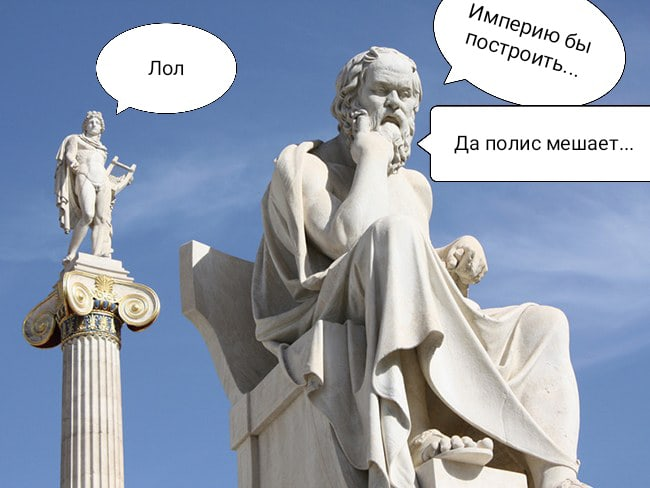
\includegraphics[scale=0.6]{regional_hehemons/161365631011485734.png}
	\label{fig:heh1} % Unique label used for referencing the figure in-text
	%\addcontentsline{toc}{figure}{Figure \ref{fig:placeholder}} % Uncomment to add the figure to the table of contents
	%	\caption{Подааарочки!!	}
\end{figure}

\section{CHAD Frontier}


Итак, у вас есть следующие преимущества:


1. Вы вот только что родились из пустоты, в отличие от более пожилых коллег. Их история это метод проб и ошибок, долгое и не всегда верное органическое развитие без особого плана и сметы. От этого они несколько перекосоебленные. Тогда как вы, используя их опыт, а может, и прямо приглашая правильных политтехнологов из Центра, можете сразу, ещë на этапе котлована, всë просчитать, и потом сразу же, не тратя времени, начать масштабировать и расти в геометрической прогрессии. Рим, вон, в Лации трахался четыреста лет от основания города, а потом нащупал верный вектор, сожрал царей, забалансил внутренние конфликты и попер в отжор, ни в чем себе не отказывая. Думаете греки тупые и просто до такого не додумались? Вы не правы, вся эта республиканская мишура греками же и придумана. Но осуществить еë в самой Греции было прост невозможно, там органическое развитие, там уже вот так вот сложилось, как есть, и любого реформатора сожрут с потрохами. Поэтому реформаторы, те, которые серьезные, они в основном на периферию и двигают, там хоть работать можно. Завоевать себе небольшую страну, и начать в ней своë видение продвигать. В Элладе жи даже какой-нибудь поселок нормально не отреформируешь. Ну, в общем, это понятно любому человеку, решившему в старом и сложившемся коллективе ченить всерьез поменять. Даже если надо, даже если сейчас явно плохо и даже если по другому явно будет лучше. Понимания всë равно не будет. Вот поэтому Фронтир - поле экспериментов, и когда эксперимент особенно удачный, то оттуда выползает какой-нибудь хтонический пиздец типа Римской Республики и жрет всë живое за две сотни лет, например.


2. В Центре Мира живут Серьезные Люди и Решают Вопросы, а вы в своем Лации крадете у соседей сабинянок, чтоб было кого того самого. Тоесть вы занимаетесь какой-то незначительной с точки зрения Центра херней, и ей же и являетесь. И отслеживать вас, во-первых, скучно, а во-вторых, некогда, надо следить, чтобы другие Серьезные Люди не выпустили кишки. Вот и получается, что удачно выкинувшая кубики периферийная шолупонь в вашем лице получает не только кучу всего придуманного центром под ключ, и минимальное внутреннее противодействие. Дык ещë и фору лет в пятьдесят-сто, так как Серьезные Люди сначала вас не замечают, потом смеются над вами, потом думают, что вы сами помрете, потом спорят кому из них вас сдерживать... А потом вы приходите к ним домой с легионами и всë, уже поздно.


3. Ну и, канешн, Фронтир. Третья имба в колоде. Вот вы выросли себе, оперились, отожрались на непосредственных соседях, Центр вас покашто не замечает. Чего делать? Масштабироваться, канешно же. Чем ближе к Центру, тем больше будет сопротивление, а самому навлекать себе на голову наказания яростные от сильных мира сего, провоцируя их на войну - зачем оно? Лучше пойти жрать галлов. Они ничейные, бегают там себе, агукают, слюни пускают. А прокачавшись на галлах и других соседушках, можно и на чей-то праздник жизни вломиться уже. Именно наличие Фронтира позволяет Периферийной Империи войти в полную силу.


И всë. Очень просто жи. Вы молоды и со старта качаетесь по имбовому билду, а не как бык поссал. Вы незаметны на ранних этапах и становитесь "крысинным королем", грызя столь же неинтересных Центру неудачников. Набрав жирка, вы жрете свой Фронтир, и только набрав массу - кидаете вызов реально серьезным игрокам. Профит.

\section{Virgin center}
Мне нужно объяснять, почему Эллада в это не смогла? Ну, во-первых, у них не было ничего из вышеперечисленного, а во-вторых — этого достаточно. Реально достаточно, если не усложнять. И мне не особо нравится привычка лепить в этом, одном из ключевых вопросов антички, кучу зауми про полисы. Вообщет что Афины, что Спарта, два ключевых гегемона Эллады, были по сути своей вполне унитарными. Остальным да, они не дали до этого дорасти, но сами-то доросли. Аттика и Лакедемон - государства, а не полисы. Но они центральные государства, а значит они, в строгом соответствии с вышеперечисленным:


1. Старые как говно мамонта и в принципе не реформируемые в плане исходного кода. Там путанная и, для стороннего наблюдателя, довольно-таки идиотская внутренняя структура, и нет кнопки, чтоб это исправить.


2. У всех на виду, и мало того, что дерутся между собой и осаживают всякие Фивы с Коринфами, дык ещë и от варваров отмахиваются. Ну и персы, канешн, следят за ними, хоть вполглаза.


3. У них нет Фронтира как такового. И даже засрав своими колониями всë Средиземноморье, его не получается получить. Это просто расширяет зону конфликта ещë сильнее, из-за чего Спарте и Афинам приходиться драться гденить около Сицилии, вместо того чтобы прост поделить мир на две части и расползтись по сторонам фармить крипов.


И всë, и больше ничего не надо. А теперь два примера того, как периферийная имперка захуярила Элладу, после чего я вас оставлю переваривать услышанное. 

\begin{figure}[h!tb]
	\centering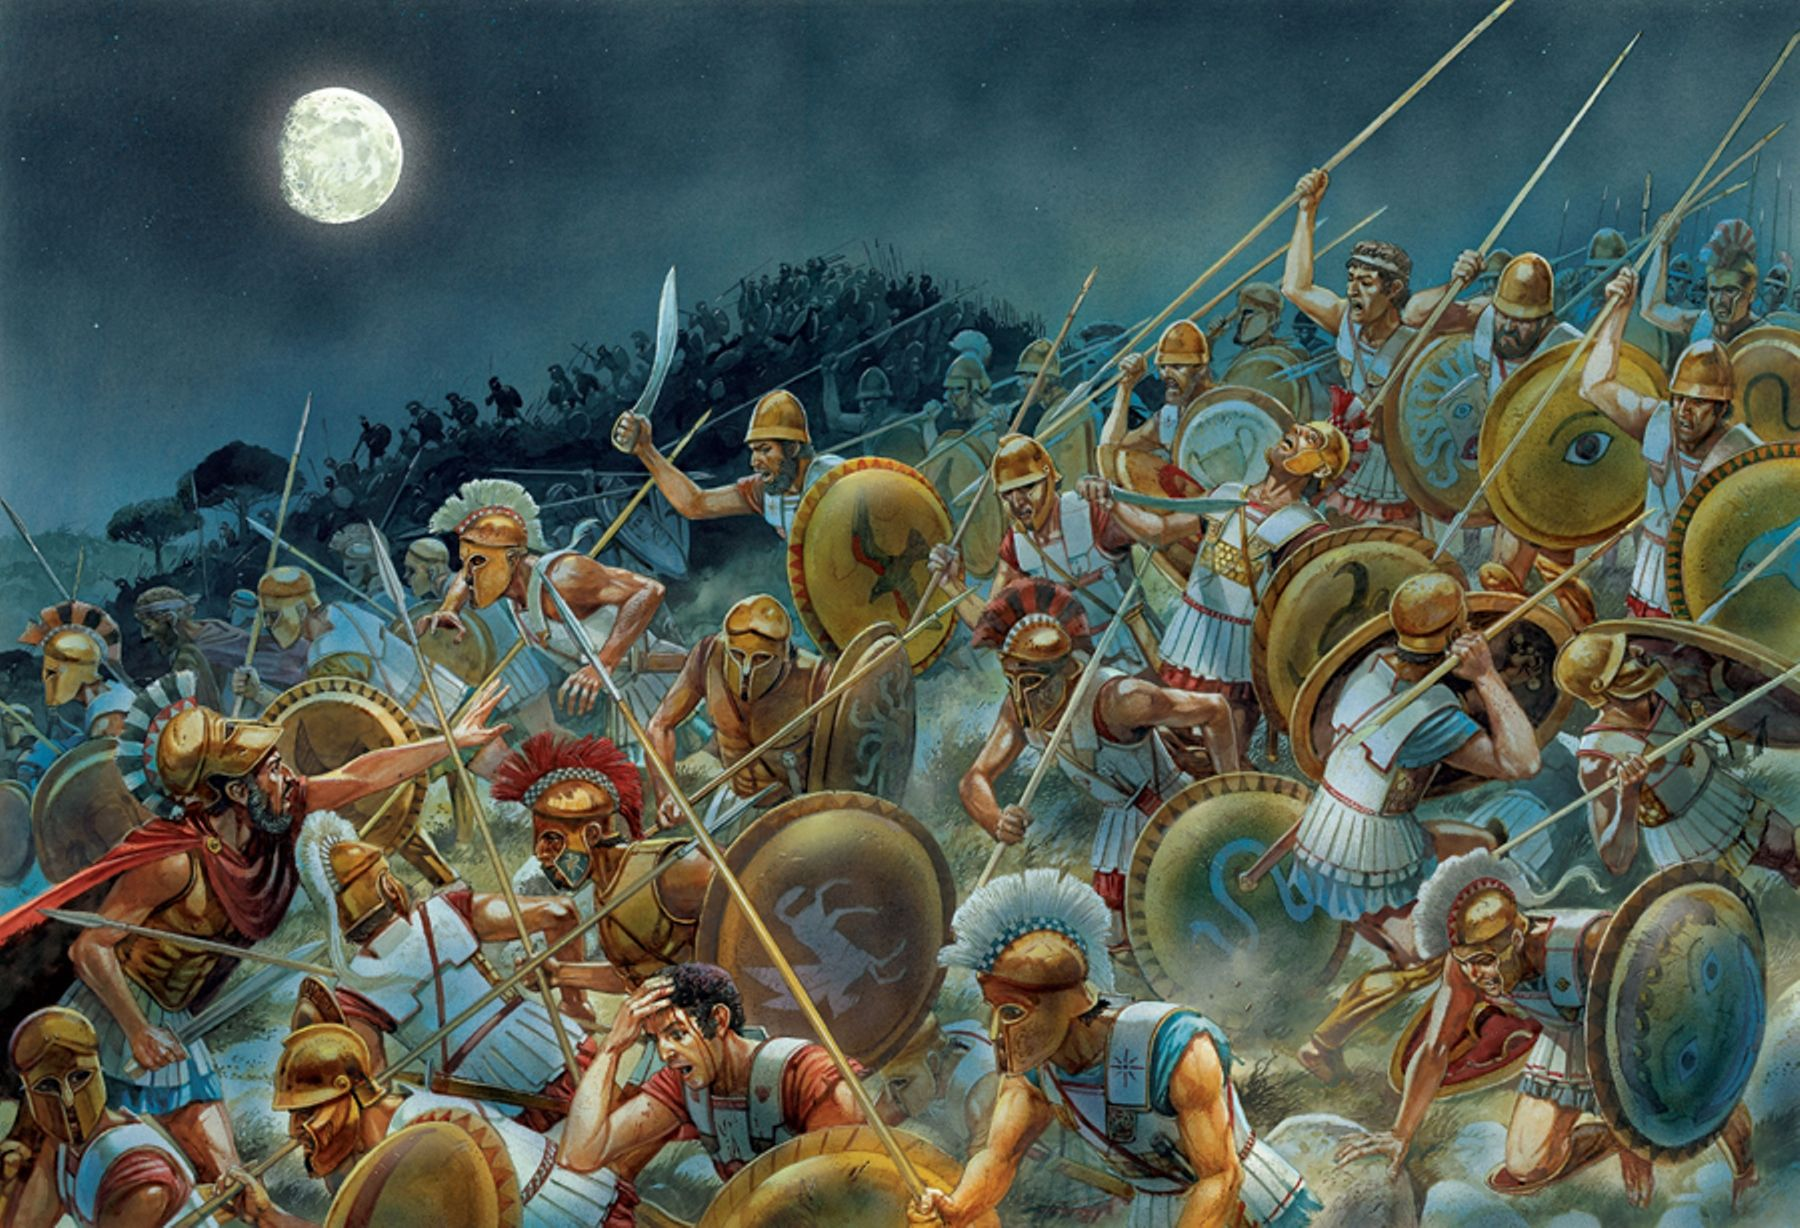
\includegraphics[scale=0.2]{regional_hehemons/1613656143131456586.png}
	\label{fig:heh2} % Unique label used for referencing the figure in-text
	%\addcontentsline{toc}{figure}{Figure \ref{fig:placeholder}} % Uncomment to add the figure to the table of contents
	%	\caption{Подааарочки!!	}
\end{figure}

\section{Как Македония сожрала Центр}
Тут мы видим воистину реактивный рост, за одно поколение. А за второе, уже руками Сашки Македонского, эллины пойдут пожирать весь мир. Но нас тут это не интересует.

Интересует нас то, что начинал Филипп Македонский заложником в Фивах, не самом сильном городе Эллады. А его страна медленно разваливалась. В конце концов предыдущего царя просто убили иллирийцы у него же дома, настолько всë было плохо. Но Филипп сумел навести порядок сначала в армии, потом в Македонии, а потом и на Фронтире, используя всякие крутые военные и гражданские новаторства, которые у тех же греков и перенял. При этом, как по учебнику, его сначала не замечают, а потом очень невнятно ему противодействуют. Как раз за несколько десятилетий до описываемых событий Спарта, Фивы и Афины были жестко опиздюлены друг другом и сопутствующим квартетом, установилось некоторое равновесие. Такое равновесное, что Филипп прям хперед носом Центра, практически не скрываясь, готовился этот центр сожрать, а греки не делали ничего, пока суммарная мощь Филиппа не выросла настолько, что превысила суммарную военную мощь Эллады. И всë, гейм овер. Македонцы берут Грецию просто как приз, без особого сопротивления, и делают эпичный дранг нах остен.
\begin{figure}[h!tb]
	\centering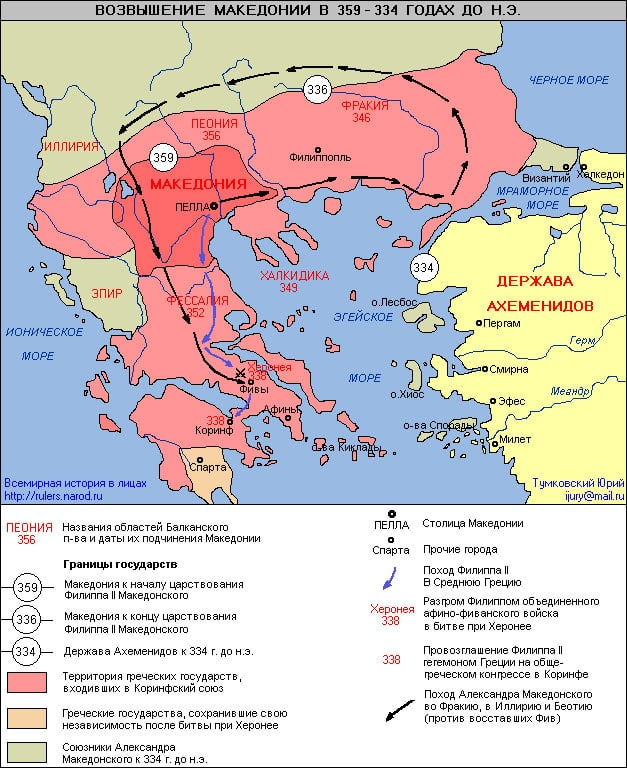
\includegraphics[scale=0.4]{regional_hehemons/1613656499119414977.png}
	\label{fig:heh3} % Unique label used for referencing the figure in-text
	%\addcontentsline{toc}{figure}{Figure \ref{fig:placeholder}} % Uncomment to add the figure to the table of contents
	\caption{Македония при Филиппе жрет Грецию}
\end{figure}
\section{Как Рим сожрал Центр}

Вот тут история поинтереснее, она многоэтапна и куда более эпична. Ну и за ней вы, собственно, и пришли, я полагаю. Итак, на Лации просыпается пока ещë маленький, слабенький и тупенький будущий Периферийный Гегемон...

\begin{figure}[h!tb]
	\centering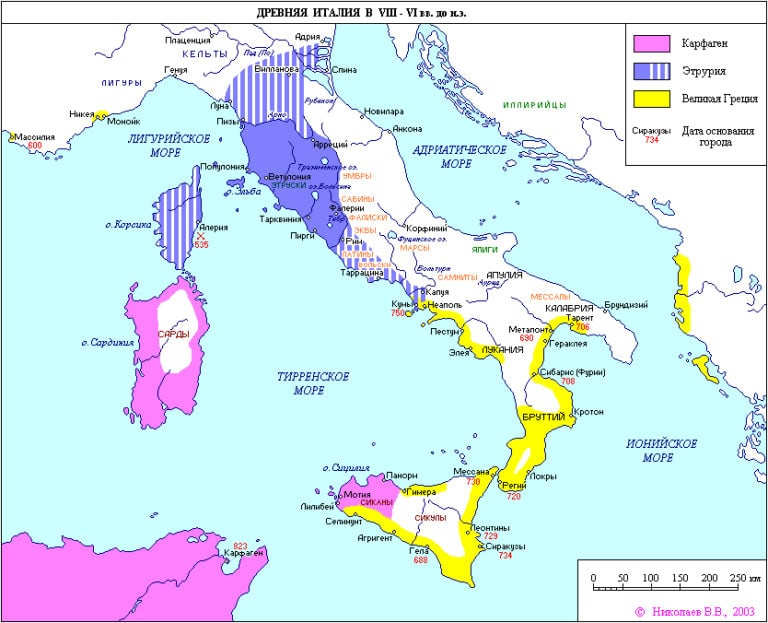
\includegraphics[scale=0.4]{regional_hehemons/1613656334110444030.png}
	\label{fig:heh4} % Unique label used for referencing the figure in-text
	%\addcontentsline{toc}{figure}{Figure \ref{fig:placeholder}} % Uncomment to add the figure to the table of contents
	\caption{Шестой век до н.э. Рим крутит хвосты коровам между греками и этрусками, в регионе первичный бульон.}
\end{figure}

Ну, первые лет четыреста он просыпается с большим скрипом, ворочается, говорит "мне сегодня ко второй", терпит былинные отказы от всяких поселков неподалеку, его сдигают галлы, в общем — ничего не предвещает беды. Однако мы уже на этом уровне видим всë то же самое, что и выше - роль периферии и преимущества отстающего. Это и новаторская, потыренная у греков с этрусками политическая система, идеальная для масштабирования до бесконечности, и периферийность (центр "сапога" и "жопа мира" в те годы - синонимы), и почти полный игнор со стороны что этрусков (которых щемят галлы) что греков (для которых Великая Греция - периферия, но центр приложения усилий - в Элладе). Это дает нашему подопечному быстрый старт. Его никто не замечает, он жрет сначала этрусков, а потом и греков. За тех пытается вписаться Пирр, сам - житель окраины эллинистического мира, и оттого сумевший столько дел натворить. Но его забарывают, канешн. А дальше - первый серьезный вызов - точно такой же периферийный гегемон.


Тут надо отвлечься и сказать "чо там у эллинов" перед Первой Пунической. После того, как Сашка устроил свои великие завоевания, эллинистический мир расширился, и Эллада перестала играть роль Центра Мира. Поэтому теперь уместно говорить о Центре как о всëм Восточном Средиземноморье. И тут у нас появились три могучие империи:

\begin{itemize}
	\item Империя Севера - собственно, Македония и подчиненная ей Греция.
	\item Империя Востока - Селевкиды и их вассалы
	\item Империя Юга - Птолемеи
\end{itemize}


А вот Империи Запада не было. Карфаген был далеко и был выключен из этого созвездия, а попытки Пирра запились себе уютную имперку сломались об уже набравший сил Рим. Вот вломился бы туда не он к моменту доедания Римом сапога, а сам Сашка Македонский на поколение раньше, и не было бы никакого Рима, можете запомнить этот твит. Причем Сашка и собирался этим заняться, судя по всему. Но умер, а потом как-то уже не до того было всем. Ну, вы знаете, все эти войны за его наследие, какие тут римляне, вообще не до них. 

\begin{figure}[h!tb]
	\centering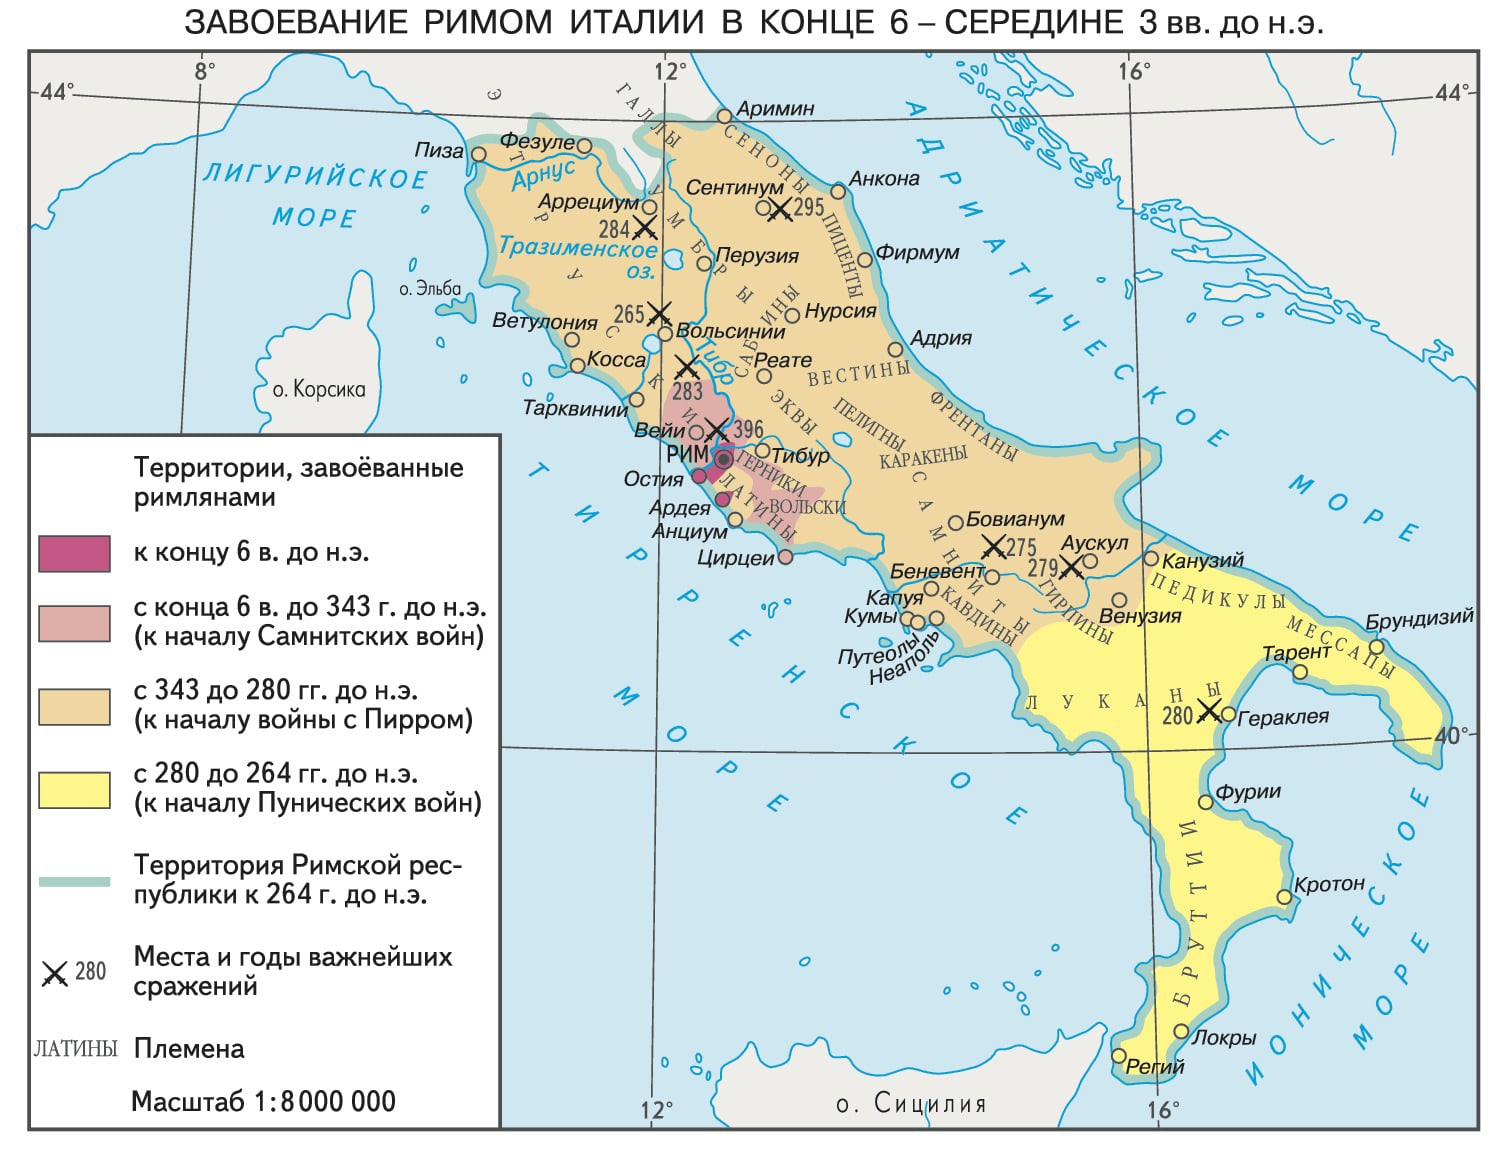
\includegraphics[scale=0.3]{regional_hehemons/1613656352188889603.png}
	\label{fig:heh5} % Unique label used for referencing the figure in-text
	%\addcontentsline{toc}{figure}{Figure \ref{fig:placeholder}} % Uncomment to add the figure to the table of contents
	\caption{Рим пошел в отжор. Обратите внимание на темп}
\end{figure}

Вот в это окно Империи Запада и влез Рим. Но по-хитрому. Пользуясь тем, что в эллинистическом мире всем не до него, он сначала отжирает себе Фронтира сколько может, а потом прет на Сицилию, врубаясь в сложнейшую для себя Первую Пуническую. Это была, неиллюзорно, битва за мировое господство. И, спустя двадцать лет, пунны признали поражение и отдали острова. После чего Рим получил выход в море, и продолжил грызть фронтир, зализывая раны. После чего злую шутку сыграла география. Двадцать лет паузы это солидно, и Карфагену бы тоже не помешало приятно округлиться, но... пустыня. Де-факто, в Африке у Карфагена не было Фронтира и некуда было расширяться. И пришлось уходить в Испанию. Тоесть осваивать Фронтир на глазах у римлян, что резко снижает эффективность. Потом случается вторая война, которая, несмотря на гений Барки, была скорее "походом обреченных". К еë началу Рим был сильнее себя времен первой войны, и значительно сильнее Карфагена. И победил. Сожрав вообще всë, что было западнее Греции. 


\begin{figure}[h!tb]
	\centering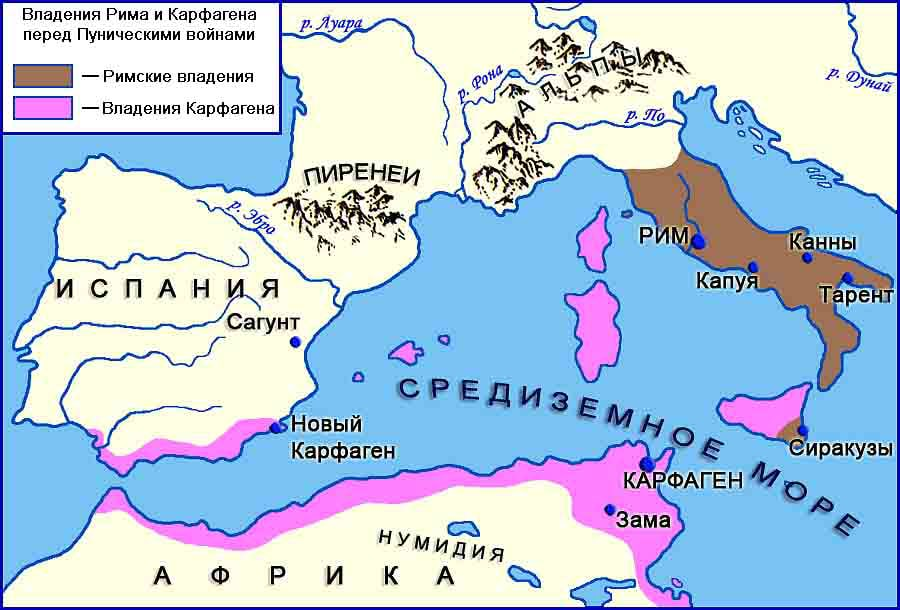
\includegraphics[scale=0.4]{regional_hehemons/1613656370149685122.png}
	\label{fig:heh6} % Unique label used for referencing the figure in-text
	%\addcontentsline{toc}{figure}{Figure \ref{fig:placeholder}} % Uncomment to add the figure to the table of contents
	\caption{Первое столкновение с Карфагеном. Обратите внимание на Испанию. Карфаген засрал еë колониями, но не более того. }
\end{figure}

\begin{figure}[h!tb]
	\centering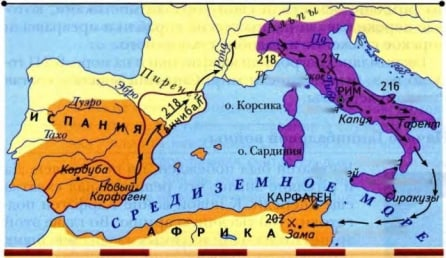
\includegraphics[scale=0.6]{regional_hehemons/1613656400130734638.png}
	\label{fig:heh7} % Unique label used for referencing the figure in-text
	%\addcontentsline{toc}{figure}{Figure \ref{fig:placeholder}} % Uncomment to add the figure to the table of contents
	\caption{Вторая Пуника, через 20 лет после первой. Забрав в прошлой войне море и острова, Рим выходит к Альпам. Карфаген же жрет Испанию. Но он уже обречен. }
\end{figure}

\begin{figure}[h!tb]
	\centering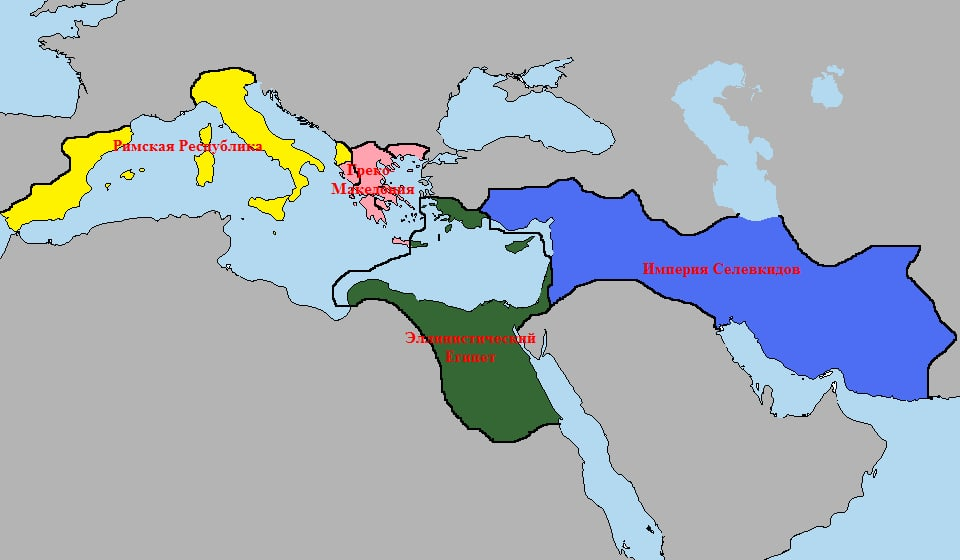
\includegraphics[scale=0.3]{regional_hehemons/1613656424143275900.png}
	\label{fig:heh8} % Unique label used for referencing the figure in-text
	%\addcontentsline{toc}{figure}{Figure \ref{fig:placeholder}} % Uncomment to add the figure to the table of contents
	\caption{Конец Второй Пуники, 201 год до н.э. Карфаген заперт в Африке и сломан. Обратите внимание на желтое пятнышко на Балканах. Да, это пиздец для Македонии, всë так.  }
\end{figure}
\begin{figure}[h!tb]
	\centering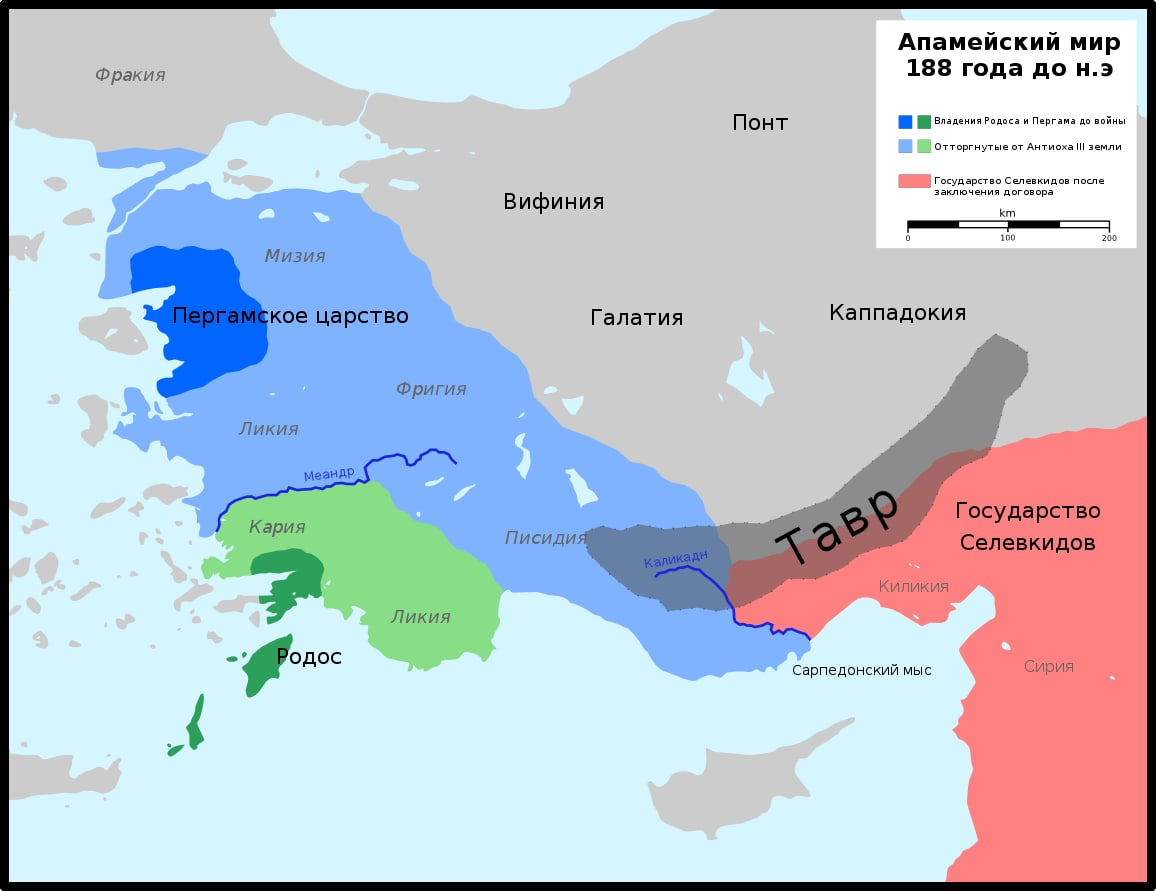
\includegraphics[scale=0.4]{regional_hehemons/1613656445174137735.png}
	\label{fig:heh9} % Unique label used for referencing the figure in-text
	%\addcontentsline{toc}{figure}{Figure \ref{fig:placeholder}} % Uncomment to add the figure to the table of contents
	\caption{188 год до н. э., Рим убивает Селевкидов. Партия.  }
\end{figure}
А что наш Центр Мира? Он... просто проспал появление сверххищника с запада. Только ко Второй Пунической Македония начинает дергаться в сторону вмешательства, да и то как-то вяло, неспешно, будто впереди целая жизнь. Но нет, впереди Первая, Вторая и Третья Македонские войны, не оставившие от Империи Севера камня на камне за несколько десятилетий. В принципе, это неудивительно, македонцам достались греки (тоесть "болезни центра" там были особенно ярко выраженными) и не было нормального Фронтира. А дальше всë. Между Второй и Третьей Македонскими Рим походя ломает Селевков в одном сражении, после чего те начинают разваливаться с чудовищной скоростью. А оставшиеся в одиночку Птолемеи ливают катку, схлопнув свою внешнюю политику и покорно ожидая, когда Рим за ними придет. Флаулесс Виктори.

\begin{figure}[h!tb]
	\centering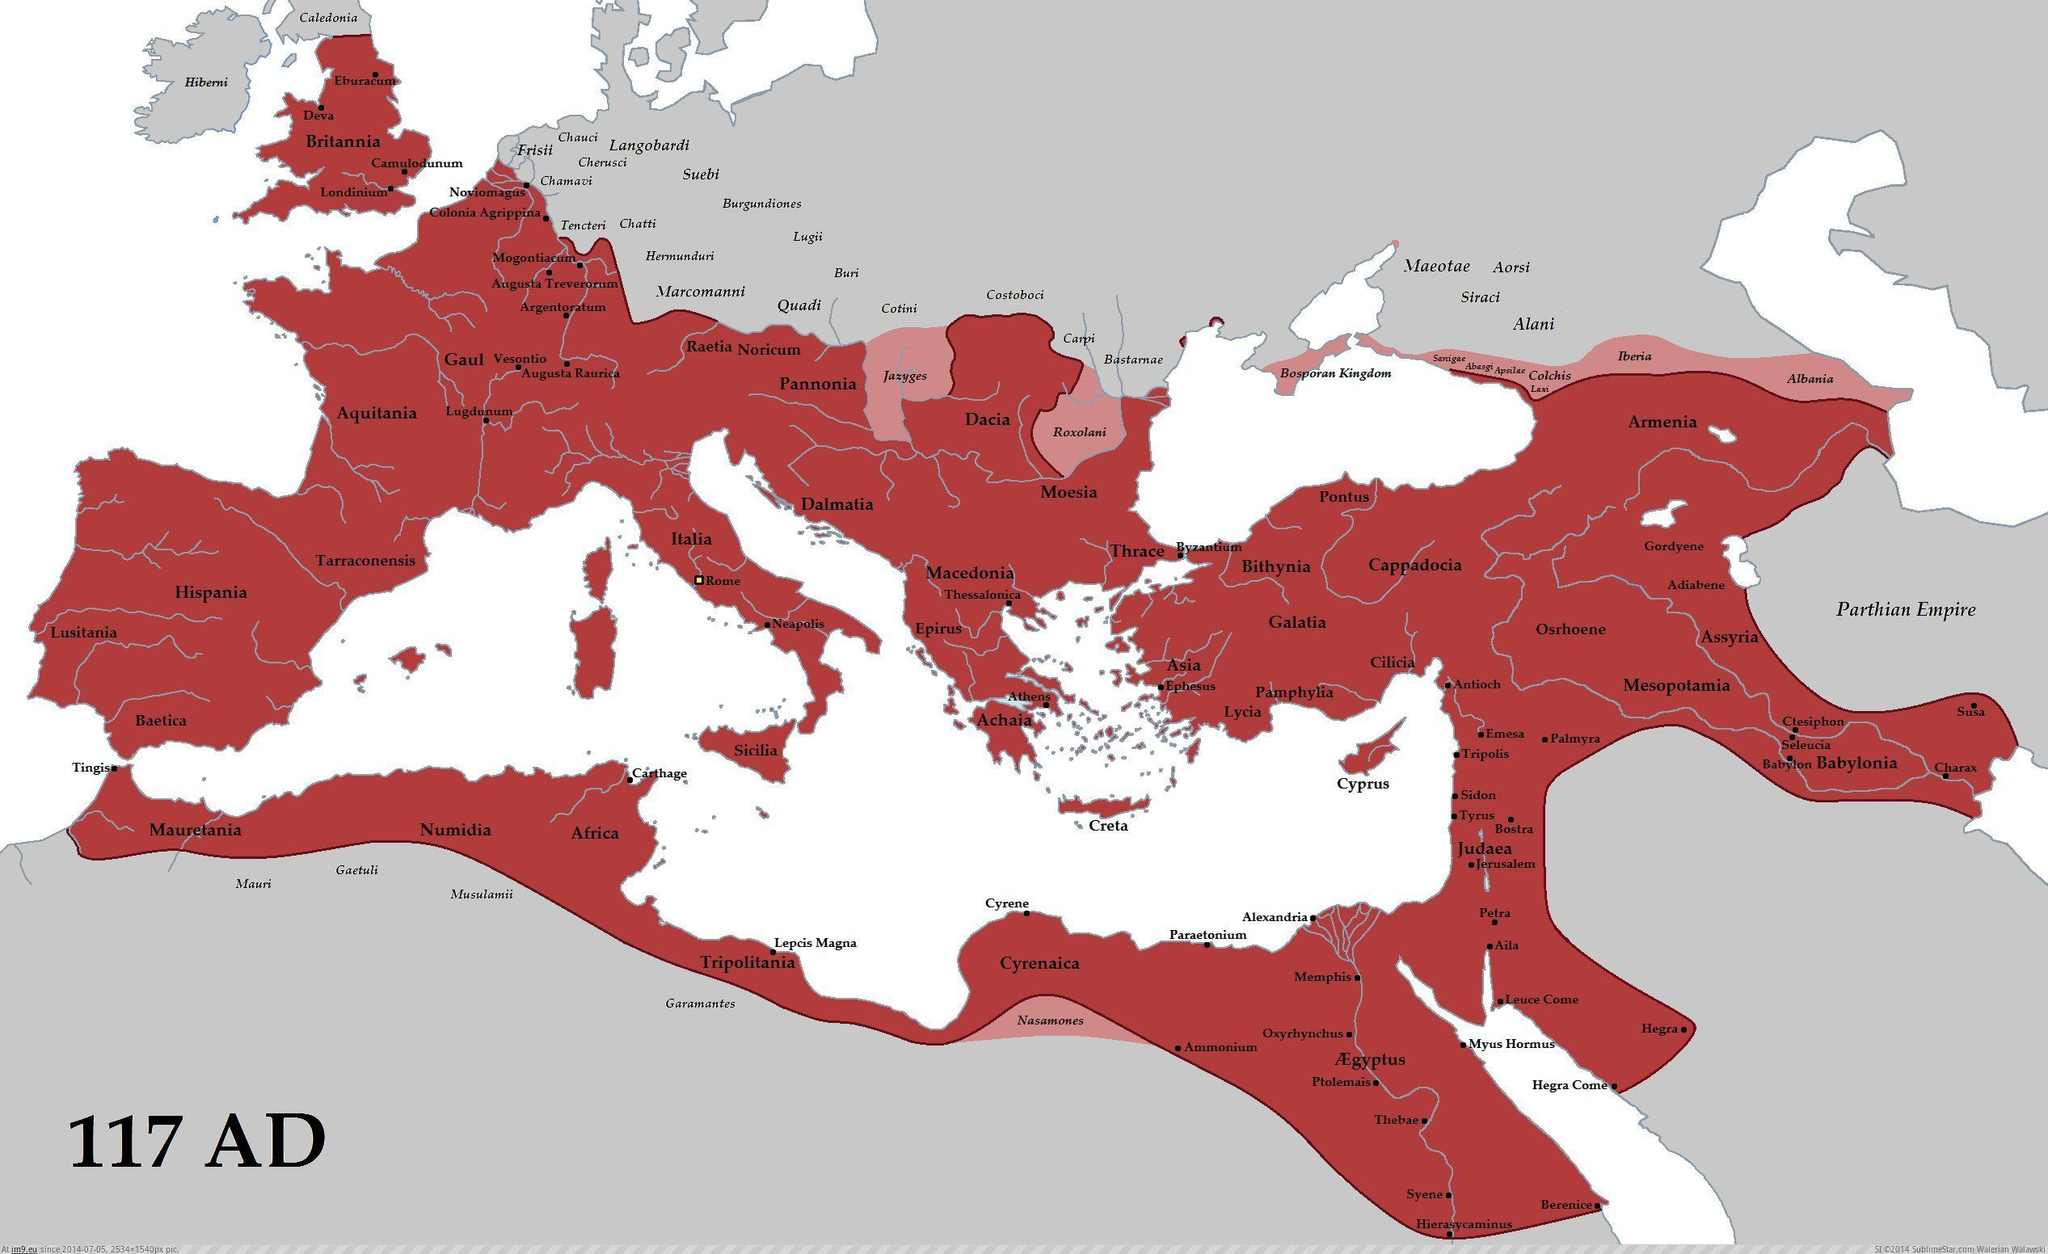
\includegraphics[scale=0.25]{regional_hehemons/1613656483182828728.png}
	\label{fig:heh10} % Unique label used for referencing the figure in-text
	%\addcontentsline{toc}{figure}{Figure \ref{fig:placeholder}} % Uncomment to add the figure to the table of contents
	\caption{Финальная сборка римского мира.  }
\end{figure}

\section{И \sout{примкнувший к ним} Митридад}
Такие дела. Надеюсь стало понятнее. А чтобы не прослыть душным римским патриотом, укажу, что и сама Республика времен расцвета сталкивалась с теми же проблемами. И хоть она их и решала, но крови те попили изрядно. Примером реактивного появления периферийного гегемона служит Митридат. Если вы вспомните как он вылез из ниоткуда, как его все проспали и сколько крови понадобилось чтоб его сломать, то увидите в нем "Филиппа, который не смог". Пример ползучей экспансии это Парфия, разжиревшая на вовремя не сожраном трупе Селевкии, и с которой Риму воевать до своей естественной смерти. Тоесть ничего уникально римского тут нет. Римляне построили имперку, томушта были периферийным гегемоном, а греки еë не построили, томушта им не были. А не потомушта римляне это римляне, а греки это греки.
\begin{figure}[h!tb]
	\centering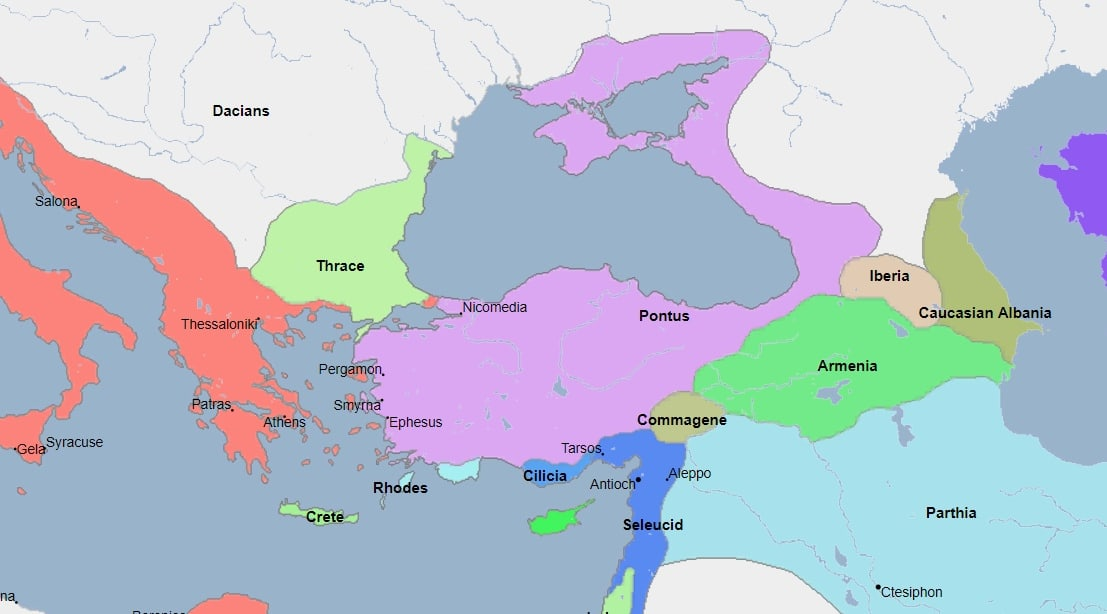
\includegraphics[scale=0.3]{regional_hehemons/1613656552160570947.png}
	\label{fig:heh11} % Unique label used for referencing the figure in-text
	%\addcontentsline{toc}{figure}{Figure \ref{fig:placeholder}} % Uncomment to add the figure to the table of contents
	\caption{Митридат и его периферийный гегемон наглядно. Неудачно, но тем не менее. Рядом отожравшаяся на трупе Селевкидов Парфия. }
\end{figure}

У меня всë. 